%#BIBTEX /usr/texbin/pbibtex -kanji=utf8 abstruct
\documentclass[10pt,a4j]{jarticle}
\pagestyle{headings}
\usepackage[dvipdfmx]{color,graphicx}
\usepackage[dvipdfmx,bookmarks=true,bookmarksnumbered=true,bookmarkstype=toc]{hyperref}
\AtBeginDvi{\special{pdf:tounicode 90ms-RKSJ-UCS2}}
\AtBeginDvi{\special{pdf:tounicode EUC-UCS2}}
\usepackage{times}
\usepackage{ascmac}
\usepackage{lscape}

%excel2latex用に追加
\usepackage{multirow}
\usepackage{bigstrut}

\begin{document}

%% 表紙
\thispagestyle{empty}
\vspace*{2cm}
\begin{center}
\LARGE
博士(工学)論文概要\\[2cm]
テスト対象の機能構造とデータの入出力情報を使ったブラックボックステスト手法の研究\\[8cm]
システム情報工学研究科 リスク工学専攻\\[1cm]
湯本剛 \\[2cm]
2017年 10月
\end{center}

%% 目次
\clearpage
\tableofcontents

%% 本編
\pagebreak \setcounter{page}{1}
\pagenumbering{arabic} % 1,2,3

\section{緒論} \label{chap:1}
ソフトウェア開発の中の品質を確保する主要な技術として,ソフトウェアテストがある.
求められるテストケースの数は,昨今のソフトウェアの複雑性と規模の急激な増加に伴い増加の一途をたどっている.
ブラックボックステストの場合,ソフトウェアの規模とテストケース数の関係は,ファンクションポイント総計値の1.15乗から1.3乗となる\cite{jones1998estimating}.また,開発プロジェクトのファンクションポイント総計値は1970年から2000年までの30年間で約10倍の増加を示している\cite{longstreet2000}.

日本におけるテスト工数の割合は開発工数全体の28パーセントから35パーセントを占めるケースが多いが,90パーセントを超えるケースもあるという調査結果が出ている\cite{IPA2015}
また,テストケースを作成する工数は,平均的にテスト工数全体の40パーセントだと言われている\cite{van2013tpi}.
これは,テストケースの開発に多くの人員が必要となることを示している.
多数の人員がテストケースを作成する工程に必要とされているにもかかわらず, テストケースを作成するための明確に定義されたルールがないために,投入された人員は個々の考え方に基づいてテストを開発することが多い.
これはテストケースの重複や漏れの原因となり,テストの活動がソフトウェアの品質を確保する役割を果たせないばかりか,コスト増や納期遅延の原因となってしまう.
本研究では,テストケースを作成する工程に投入される人員が、必要なテストケースを網羅的に抽出し,抜け漏れを防止できるようにすることを目的とし,適切な数のテストケースを開発するための手法を提案し,その適用評価を行う.

本論文は6章で構成される. 
2章では,研究対象とシステムテストにおけるブラックボックステストにおける課題と,関連する先行研究について述べる.また,本研究で使用するテスト分析手法について解説する.
3章では,前章で述べた課題を調査するために実験を行い実験結果で確認を行う.
4章では,テストデータの入出力に着目し、テスト分析を網羅的に行う手法の提案と適用評価を行った.
5章では,テストデータの入出力を2回必要とするテストケースに対して,重要な処理順序の組み合わせを抽出する方法の提案と適用評価を行なった.
最後の6章では,結論を述べる.



\section{複数人でテストケースを作成する課題} \label{chap:2}
\subsection{本研究の対象となるテストケースの開発方法とテストレベル} \label{sec:2-1}
\subsubsection{テスト開発プロセス}
テストのプロセスは, テスト計画がVモデルの左側の活動と並行に行われ,その後時系列にテスト分析,テスト設計,テスト実装が行われた後,Vモデルの右側の活動の中で,テスト実行と終了基準の評価が行われる.
このプロセスは,Vモデルであらわす各レベルごとに行われる.システムテストレベルであれば,システムテストレベルのテストプロセスが必要となる.
テストのプロセスの中でテスト分析,テスト設計,テスト実装の3つのテストケースを作成するための活動はテスト開発プロセスと呼ばれている[5] .
テスト分析では,テスト対象をテスト設計ができるサイズに詳細化する.
このアウトプットはテスト条件と呼ばれている.
このテスト条件を合理的にある基準で網羅する方法を考える行為がテスト設計であり,そのための技法をテスト設計技法と呼ぶ.
テスト設計のアウトプットはテストケースである.

\subsubsection{テストケースを開発する方法}
テストケースを開発する方法は,ソフトウェアの物理的な構造を基にテスト設計するホワイトボックステストと,ソフトウェアの仕様を基にテスト設計するブラックボックステストに大別できる\cite{myers2011art} .
本研究では,ブラックボックステストを対象とする.
テスト対象そのものではなく,テスト対象の動作条件や論理的な振る舞いの記述がベースあるがゆえに,ベースとなる情報からテストケースにしたてるまでの詳細化が複数の解釈で行われることが多くなるためである.
%テストベースがAUTの物理的な構造ではなく論理的なふるまいの記述であるがゆえに,テストを作るための詳細化が複数の解釈で行われることが多い\cite{yumoto2013test}.

\subsubsection{テストレベル}
ソフトウェアテストは,開発ライフサイクルの中で複数のテストレベルに分けて行われる.
各テストレベルはソフトウェア開発の段階的詳細化のレベルと対応している.
本研究は,複数のレベルの中で,システムレベルで行われるブラックボックステストに焦点を当てている.
システムレベルのテストは,開発した単体のソフトウェアがすべて統合されるため,規模の増大と複雑性の増加の影響を直接的に受けるからである.


\subsection{システムレベルでのブラックボックステストの課題} \label{sec:2-2}
\subsubsection{システムレベルでのテスト分析の課題}
テスト分析の活動の出力となるテスト条件は,機能,トランザクション,品質特性,構造的要素といった多くの側面の総称である.
テスト対象の詳細化をするときの起点や中間分類が混乱しないように各側面の関係を整理するための構造化が必要である.
しかし,テスト分析におけるテスト条件群の構造化は,研究や実務においても,経験則や個人の考え方に基づく構造化に留まっている.
一般的には,テストベースを大項目,中項目,小項目と詳細化していくことが多い.
この方法は,詳細化する際の各分類項目に明確なルールが定義されていないため,個人毎の何かしらの考え方で詳細化するための分類を決めていくことになる.
そのため,複数人で作業を行うと分類にばらつきが発生し,同じテスト条件が複数の階層に現れてしまったり,同じ意味のテスト条件が別の名称で選択されるといった混乱が起きてしまう.
したがって,テスト分析が複数人で行われるときには,テスト条件の重複,もしくは完全に抜け落ちるといった可能性が高くなる.
テスト開発の最初の活動であるテスト分析にて特定するテスト条件にこのような問題があると,その後の活動で作られるテストケースの抜け漏れ,重複に影響を及ぼす.
テスト分析手法に関する研究は,Nishi [12], Akiyama[13], Yumoto\cite{yumoto2013test}がある.
しかし,複数の人数でテスト分析を行う際のテスト条件の重複と欠落について手法がどの程度有効であるかは,ほとんど研究されていない.

\subsubsection{システムレベルでのテスト設計の課題}
テストケース数の増加は,単一機能のテストより機能間の統合において問題となる。
この場合のテストケース数は,単一の機能や制御構造の和で求めるのではなく,積となるためである。
それに加え,このテストでは,状態遷移に伴う時系列の組合せのテストも求められることから,テストケース数の爆発問題が生じる。
必要なテストケースの抽出方法とその網羅性に関する研究は多々あるが,多くは機能や制御構造を基にした方法である
状態遷移間の組合 せについては N スイッチカバレージに従ってテストケースを抽出する方法がある。
N スイッチカバレージとは,状態の遷移をパスとし,N+1 個の遷移パスを網羅する基準に従て組合せテストケースを作成する。
N=0 では遷移パスの組合せをテストできないため N=1,すなわち S1 網羅基準(1 スイッチカバレージ)が必要とされている
しかし,S1 網羅基準を満たすテストケース数は, 2つの状態遷移間における遷移数の積となり,膨大なテスト工数を必要とする課題になる

\subsubsection{論理的機能構造を使ったテスト分析手法の利用}
本研究では,論理的機能構造を使ったテスト分析手法を利用して,テスト分析の課題の調査を行う.
この分析手法を採用する理由は,実験のための題材となる仕様書,模範解答が揃っているためであり,それらの題材を使って実験を行った実績があるためである.

この手法は,図~\ref{fig:D-3-Fig3}の論理的機能構造基づいてフィーチャをMECEに分解して,テスト条件を特定する.
図~\ref{fig:D-3-Fig3}に示す各箱が,各フィーチャに要求されるテスト条件を特定する有用なガイドとなる.

\begin{figure}[h]
  \begin{center}
	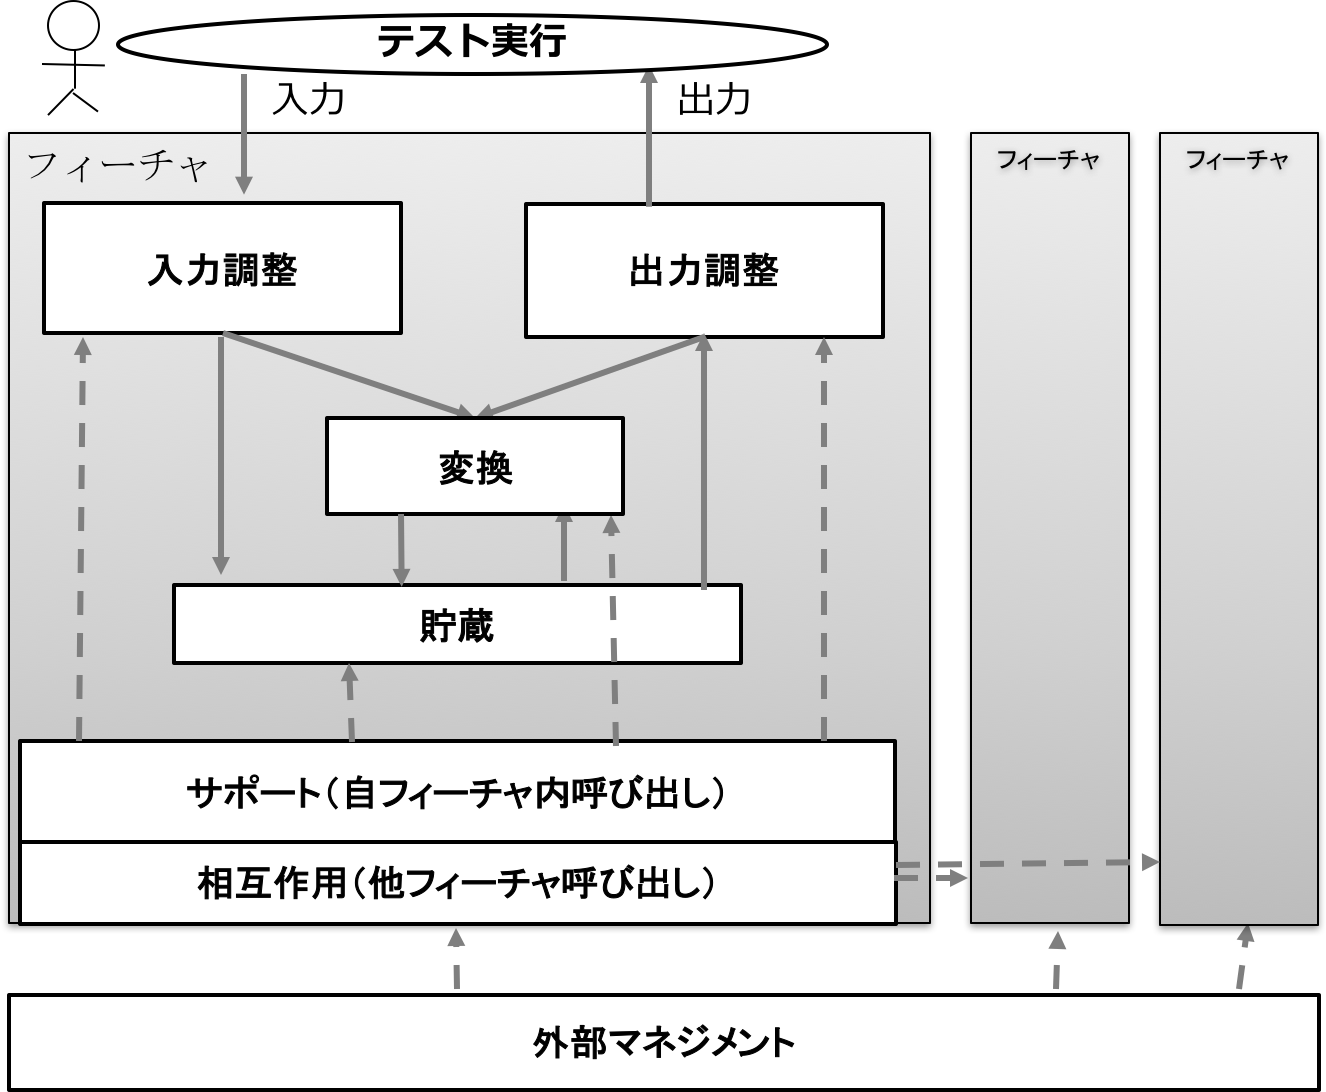
\includegraphics[width=8cm]{./image/D-3-Fig3.png}
	\caption{MECEにフィーチャからテスト条件を識別する方法}
	\label{fig:D-3-Fig3}
  \end{center}
\end{figure}

ただし,論理構造は抽象的な概念であるため,各個人の解釈に違いが出る可能性がある.
テスト条件の特定に一貫性を持たせるため, 論理構造に対してテスト対象に特化した名前付けを行う.
名前付けしたものをテストカテゴリと呼ぶ.
更に,このテスト分析手法では,テストベースからテスト条件を特定するステップも定義した。
多くのテスト開発に従事するテスト担当者がそのステップに従うと,その全てのテスト担当者は,同じルールに沿って各自の仕事を実行できる.
結果として,特定したテスト条件の重複や漏れの防止につながる.
これは本手法の主たる効果となる


%%%%%%%%%%%%%%%%%%%%%%%InSTA2016の論文%\chapter{論理的機能構造を使ったテストケースの特定方法}
\section{テスト分析でのテスト条件の抜け漏れの傾向}\label{chap:3}
\subsection{検証実験の背景} \label{sec:3-1}
これまでの研究では,同一組織内で本分析手法を導入したグループと導入していないグループでの仕様項目の選択数を比較する実験結果が得られている,
この実験にて,分析手法を導入したグループが, 導入していないグループよりも抜け漏れが少なく重複も少ない結果となった.
しかし,実験データは1組のみであり,傾向を見るためにで不十分である.
テスト分析手法を適用する前のテスト分析の傾向,及び適用後との比較結果を分析することを目的に,複数のグループに対して検証実験を行った.
検証実験は3回行った.
1回目,2回目の検証実験と3回目の検証実験は実施方法が異なるため,2つは分けて考察を行う.

\subsection{1回目,2回目の検証実験からの考察}
\subsubsection{検証実験の手順}
検証実験は,ワークショップを通じて実施した.
ワークショップでは,最初に,演習に使うテストベースを示すが,参加者が各自の考えに基づいたテスト分析を実行してもらう.
その後,4〜5名の参加者をランダムにグルーピングし,グループ内で各自のテスト分析の結果をグループの回答としてまとめる.

最初の分析結果のまとめが終わった後,テストカテゴリを用いたテスト分析手法と実施手順を説明して手順に沿って再度テスト分析を参加者が各自で実施する.
その後は最初の分析結果同様にグループの回答をまとめる.
ワークショップの一連のアウトプットを検証実験のデータとして利用した.

\subsubsection{テスト分析手法適用しないときのテスト分析の結果}

テスト分析結果のばらつきは図 ~\ref{fig:D-3-Fig1-1}から図 ~\ref{fig:D-3-Fig1-4}にて確認できる.
検証実験による典型的なテスト分析の結果を図 ~\ref{fig:D-3-Fig1-1}から図 ~\ref{fig:D-3-Fig1-4}でいくつか示す.

\begin{figure}[htbp]
 \begin{minipage}{0.5\hsize}
  \begin{center}
   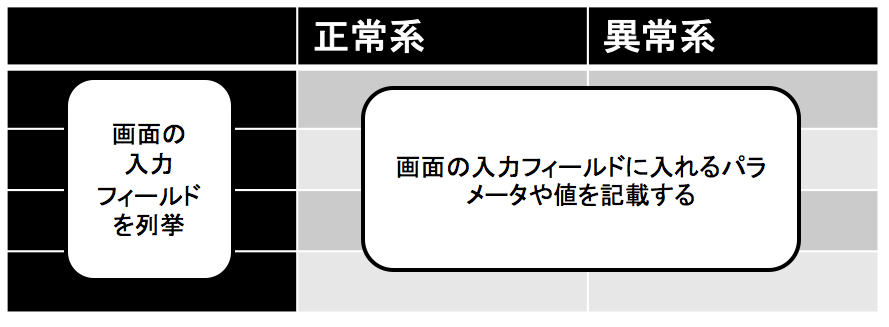
\includegraphics[width=70mm]{./image/D-3-Fig1-1.png}
  \end{center}
  \caption{テスト分析の事例:CS1}
  \label{fig:one}
 \end{minipage}
 \begin{minipage}{0.5\hsize}
  \begin{center}
   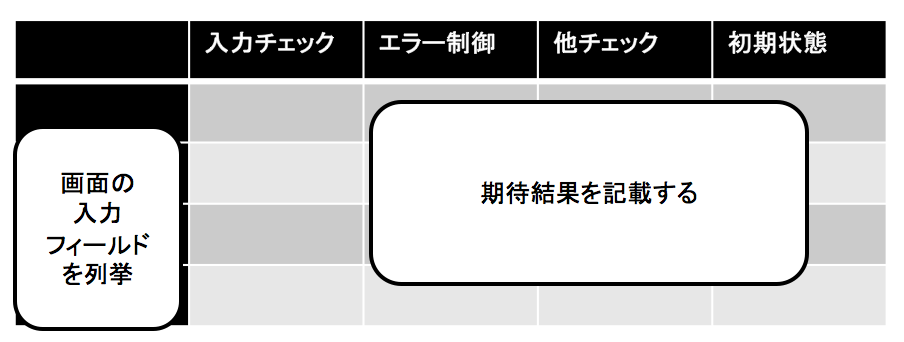
\includegraphics[width=70mm]{./image/D-3-Fig1-2.png}
  \end{center}
  \caption{テスト分析の事例:CS2}
  \label{fig:two}
 \end{minipage}
\end{figure}

\begin{figure}[htbp]
 \begin{minipage}{0.5\hsize}
  \begin{center}
   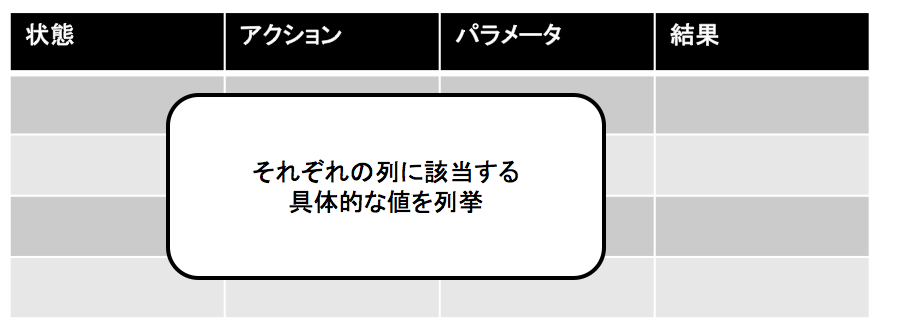
\includegraphics[width=70mm]{./image/D-3-Fig1-3.png}
  \end{center}
  \caption{テスト分析の事例:CS3}
  \label{fig:one}
 \end{minipage}
 \begin{minipage}{0.5\hsize}
  \begin{center}
   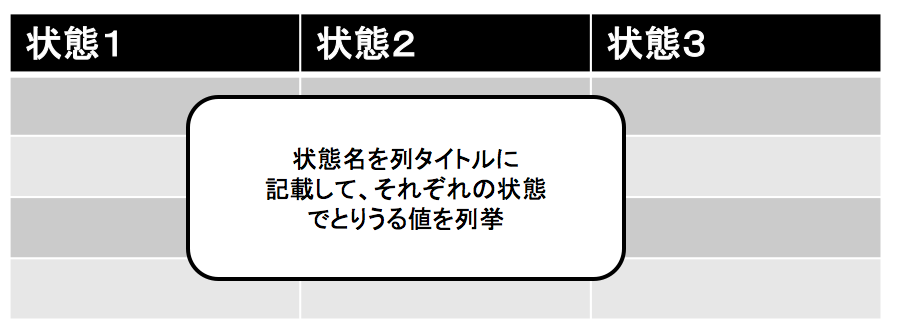
\includegraphics[width=70mm]{./image/D-3-Fig1-4.png}
  \end{center}
  \caption{テスト分析の事例:CS4}
  \label{fig:two}
 \end{minipage}
\end{figure}

\begin{enumerate}
\item CS1 と CS2:両方ともAUTの入力フィールドを行タイトルに列挙している.しかしながら列名と表の内容が異なっている.
\item CS3: 表の中に記載されている各列,アクションとパラメータと期待結果などが独立しているため,それぞれの間の関連を特定できない.
\item CS4: AUTの状態が列名として列挙されている.各状態で取りうるパラメータと値が表の中に記載されている.
\end{enumerate}
この結果は複数の個人がそれぞれ複数の結果に到達することを示している.
複数の結果とは,テスト分析を通して特定したテスト条件にばらつきがあることを意味している.
したがって,テスト分析が多くの人たちで行われるときには,テスト条件の重複,もしくは完全に抜け落ちるといった可能性が非常に高くなる.
\subsubsection{1回目と2回目の検証実験結果の評価}
1回目,2回目の実験では,グループでの回答を実験結果として利用し,8つの実験結果が収集できた.
テストカテゴリを使った手法を知らないで行った演習結果と,テストカテゴリを用いた分析手法の手順にそった演習結果とで比較をした.
実験結果の評価のために,表~\ref{tbl:D-3-tbl4}に示した評価レベルを設定した.
% Table generated by Excel2LaTeX from sheet 'Sheet1'
\begin{table}[htbp]
\footnotesize
  \centering
  \caption{評価レベルの定義}
    \begin{tabular}{|l|p{14em}|}
       \hline
    評価レベル & \multicolumn{1}{l|}{比較結果} \\
        \hline
     B    & リストした仕様項目数は増加していない, かつ実験の期待結果よりも少ない.  \\
        \hline
    -     & リストした仕様項目数は増加していない, しかしすでに期待結果と同数である.  \\
        \hline
    A     & リストした仕様項目数は増加している, しかし実験の期待結果よりも少ない.   \\
       \hline
    A+    & リストした仕様項目数は増加している, かつ実験の期待結果に達している. 仕様項目の数は増加していない,.  \\
        \hline
    \end{tabular}%
  \label{tbl:D-3-tbl4}%
\end{table}%
検証実験での評価結果は,表~\ref{tbl:D-3-tbl5}に示したとおりである.

\begin{table}[htbp]
\footnotesize
  \centering
  \caption{2つの検証実験結果の評価}
    \begin{tabular}{|l|l|l|l|l|l|l|l|l|}
    \hline
    \multicolumn{1}{|c|}{\multirow{2}[4]{*}{論理的機能構造}} & \multicolumn{8}{c|}{チーム} \bigstrut\\
\cline{2-9}          & TM1   & TM2   & TM3   & TM4   & TM5   & TM6 & TM7 & TM8 \bigstrut\\
    \hline
    変換  & B     & A     & B     & B     & B     & B & A     & A\bigstrut\\
    \hline
    入力 &  -     &   -     &   -    &   -    &   -    & -     & A     & B   \bigstrut\\
    \hline
    出力 & -     & -     & -     & -     & -     & A+ & A     & A \bigstrut\\
    \hline
    貯蔵 & -     & A+    & -     & A+    & A+    & -& A     & A  \bigstrut\\
    \hline
    サポート & B     & B     & B     & B     & B     & B& B     & A \bigstrut[t]\\
    \hline
    相互作用  & B     & A     & A     & A+    & A     & A+& B     & A \bigstrut[b]\\
    \hline
    \end{tabular}%
  \label{tbl:D-3-tbl5}%
\end{table}%

TM1からTM6までは最初の実験の結果である.
音楽生成機器がテスト対象でありテスト対象フィーチャはボリュームコントロールであった.
全チームにてテストカテゴリ内に列挙した仕様項目の数が増えており,論理構造の項目ごとの比較では,相互作用にて5チームの列挙数が増加しているが,サポートでは全チームにて増加していない.
TM7とTM8は2回目の実験であり,フライト予約システムがテスト対象で,新規飛行機予約がテスト対象フィーチャであった. 
全チームにてテストカテゴリ内に列挙した仕様項目の数が増えており,論理構造の項目ごとの比較では,変換と出力と貯蔵にて両チームともに仕様項目の列挙数が増えた.

全体的に定量的な向上が見られるが, このテスト分析手法を使うことによって特定のカテゴリに特徴的な傾向が見られるとい得ることが見つからなかった.
そのため,3回目の検証実験では,実験データ取得の方法を変更して実験を行った.

\subsection{3回目の検証実験からの考察}
\subsubsection{3回目の検証実験結果の評価} \label{sec:3-2}

3回目の検証実験では,グループ単位ではなく,各参加者の実施結果を収集し.57名分の実験結果を収集した.
ワークショップのを通して,テスト分析手法を知らない状態での演習実施、一部分だけ説明した状態で演習実施,すべて説明した状態で演習実を行い,各参加者の演習結果を実験データとして収集した.

\begin{figure}[h]
  \begin{center}
  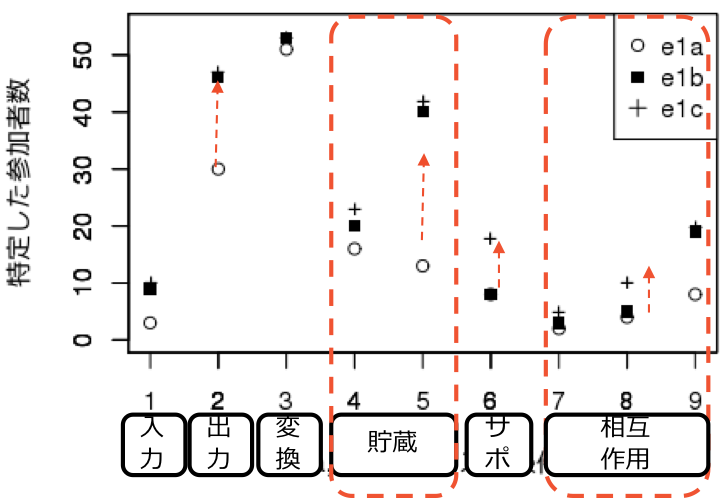
\includegraphics[width=8cm]{./image/D-3-Fig12-1.png}
  \caption{参加者あたりのテスト条件特定数}
  \label{fig:D-3-Fig12-1}
  \end{center}
\end{figure}

各参加者が特定できたテスト条件数 (回答数) を図\ref{fig:D-3-Fig12-1}のように論理的機能構造で分類して比較した.
図\ref{fig:D-3-Fig12-1}のY 軸はテスト条件毎に解答できた参加者数を示し,X 軸は,テスト条件を示している. 
1a(テスト分析手法を知らない状態での演習実施) 1b,1c と進むにつれて,分析で特定できるテスト条件が増えていることがわかる.
テスト分析手法の知識を与えることで特に伸びたのは,出力と貯蔵に属するテスト条件であった.

\subsubsection{テスト分析手法適用前のテスト分析方法}
57名のiaのときのテスト分析方法は,全てのやり方が異なっていた.
しかしその中でもテスト分析結果の記載方法は特徴があるため,図\ref{fig:D-3-Fig14}に示す通り、大きく4パターンに分類した.
\begin{figure}[h]
  \begin{center}
  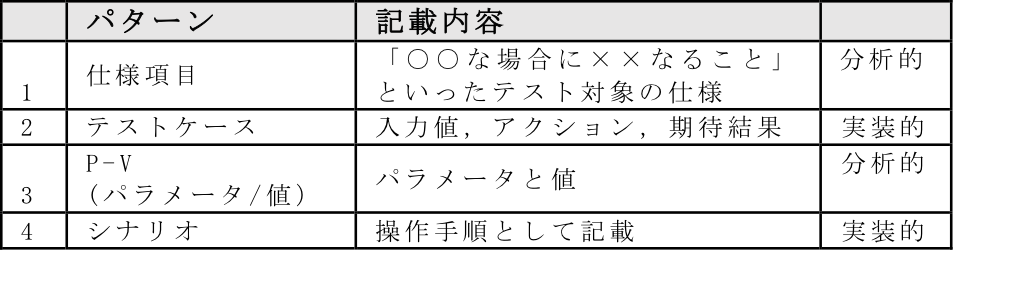
\includegraphics[width=8cm]{./image/D-3-Fig14.png}
  \caption{テスト分析パターン}
  \label{fig:D-3-Fig14}
  \end{center}
\end{figure}
この4パターンとテスト条件の特定数に相関があるかをスピアマンの順序相関分析を使って調べたが,相関があると結論付けられる値には
ならなかった.
この結果から,それぞれの分析方法のばらつきから起きる重複や欠落の課題は考えられるものの,テスト分析の違いがテスト条件を特定できるスキルとは関係ないことがわかった.


%%%%%%%%%%%%%%%%%%%InSTA2015の論文\chapter{I/Oテストデータパターンを使ったテストケースの特定方法}
\section{I/Oテストデータパターンを使った仕様項目特定の方法}\label{chap:4}
\subsection{研究の概要} \label{sec:4-1}
\subsubsection{研究の目的} \label{sec:4-1-1}
前章では,3回の検証実験を通じて,本手法の説明を参加者にすることによるテスト条件を特定できる数の向上が観察できた.
また,2章にて課題としていた,テスト分析の結果がばらつくことを実験を通じて観察することができた.
本章では,テスト分析において,テスト条件を網羅的に特定する方法として,テスト実行時のデータのI/O に着目し,テストベースを分析する際にテスト実行時のデータI/Oの要素で分解し網羅性を確認する方法を提案する.

\subsubsection{I/Oテストデータパターン} \label{sec:4-1-1}
テストを実行するためには,データをAUTにインプットし,AUTのアウトプットを期待結果と実際の結果で比較する.
テスト実行をするときのデータの入出力(以降I/Oと呼ぶ)は,パターンとして分類できる.
AUTへのデータの入力の方法は,外部からの入力,内部に保持したデータの入力,外部と内部からの入力の3パターンに分類できる.
同じようにAUTからのアウトプット方法は3パターンに集約でき,入出力の組み合わせ数はすべてで9パターンとなる.

たとえば,シンプルな機能の四則演算の計算結果が正しいことを検証するときには,AUTの外部から複数の値を入力し,AUTがそれらの値を計算し,計算結果をAUTの外部にアウトプットする.
これは「外部からのデータ入力,外部へのデータ出力」というパターンになる.

AUTに対するテスト実行時のデータの入出力をまとめたパターンは\ref{fig:D-3-Fig11}のように9パターンに集約できる.
   \begin{figure}[htbp]
 \begin{center}
 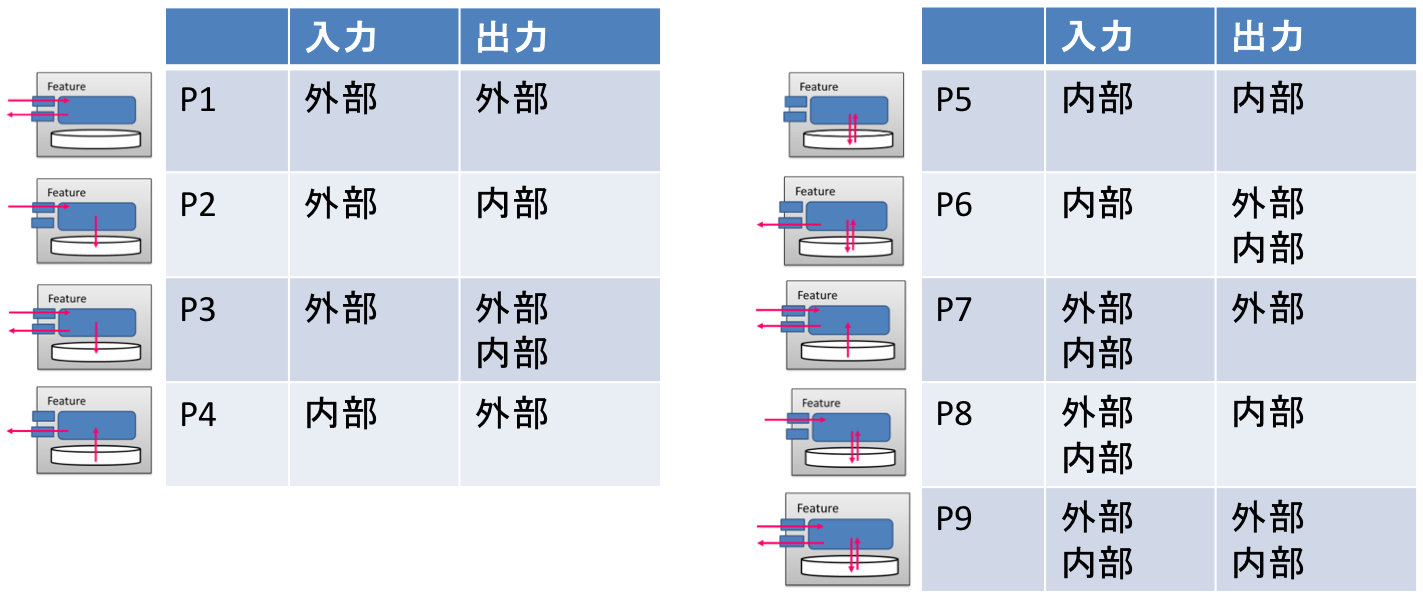
\includegraphics[width=9cm]{./image/D-3-Fig5.png}
 \caption{I/Oデータパターンの説明}
 \label{fig:D-3-Fig11}
 \end{center}
  \end{figure}
これをI/Oテストデータパターンと呼ぶ.
I/Oテストデータパターンがテスト実行時のデータの入出力から見た全体集合となる.

P1からP9のI/Oデータパターンは単一の入出力の全体像となる.単一の入出力では,論理的機能構造の入力調整,出力調整,変換,貯蔵を通過する.
P1に分類できるシンプルな四則演算の場合,外部からの入力に対して外部に出力する間に,図〜ref {fig:D-4-Fig7}のように論理的機能構造の入力調整,変換,出力調整を通過する.
この3箇所がテスト分析で特定すべきテスト条件の候補となる.
 \begin{figure}[htbp]
 \begin{center}
 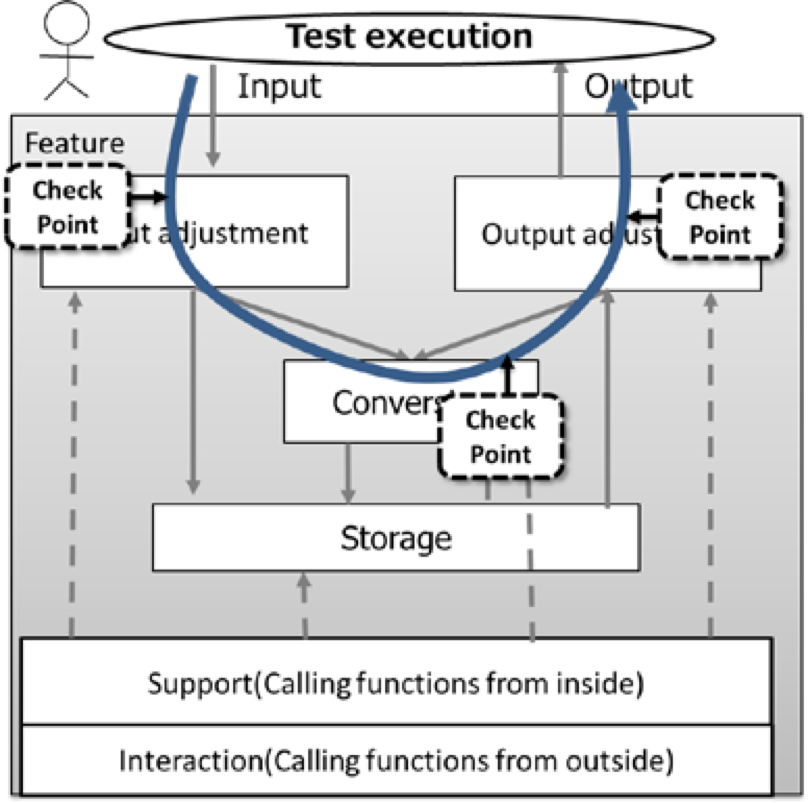
\includegraphics[width=7cm]{./image/D-4-Fig7.png}
 \caption{I/Oテストデータパターンのデータの流れ}
 \label{fig:D-4-Fig7}
 \end{center}
 \end{figure}

しかし,実際に期待結果を確認するチェックポイントは3箇所とは限らない.
なぜなら,入力調整に該当する入力の際に適切な値だけ受け入れることと,変換に該当する計算が適切に行われていることの2つだけであり,出力が適切にされることはチェックポイントとしないといったケースが考えられるためである.

\subsubsection{これまでの実験データを使った調査}
2章で行った検証実験の結果をI/Oテストデータパターンを使うとどこに分類されるかを調査し,結果を考察した.I/Oテストデータパターンと,テスト条件として特定した論理的機能構造を確認することで,各I/Oデータパターンのデータのフローの中で期待結果を確認するチェックポイントが限られていることが確認できた.

\subsubsection{サポートと相互作用に関する考察}
論理的機能構造の要素であるサポートと相互作用は,単一の入出力だけではなく,関係する他の処理の呼び出しに着目してテスト条件を特定するための分類である.
サポートは,テスト対象フィーチャでのテスト実行時のアクションによって内部的に呼び出される別の処理の結果確認のことを指している.

一方,相互作用は,テスト実行時のアクションによる副作用を,他フィーチャに対するアクションにて呼び出して確認することを指している.
サポートに該当する仕様項目の特定に使う呼び出しのきっかけと相互作用に該当する仕様項目の特定に使う呼び出しのきっかけを整理して,I/Oテストデータパターンとの対応がわかるようにした.


\subsection{I/Oテストデータパターンを使ったテスト分析の実験} \label{sec:4-2}
本章の実験では,現実のプロジェクトで作られたテストケースと,今回提案するI/Oテストデータパターンを使ったテスト分析結果を比較し,手法の効果を分析する.
\subsubsection{実験の目的} \label{sec:4-2-1}
この実験は今回提案しているテストカテゴリにI/Oテストデータパターンを使う手法が,現実のテスト設計と比較して網羅的に仕様項目を特定できることを目的とする.そのために現実のテスト設計の結果と,I/Oテストデータパターンを使った分析結果を比較する.

\subsubsection{実験の概要} \label{sec:4-2-3}

実験対象のAUTは,実在するオンラインのモバイル写真共有アプリケーションを使った.
モバイル写真共有アプリケーションの開発にて実際に使われたテストケースと、提案する手法で分析した結果を比較する.

今回の実験で使う成果物には,テストケースのみであり,テスト分析のアウトプットとなるテスト条件の一覧はなかった.
そのため,比較元のテストケースは,今回の実験のためにテスト分析でのアウトプットであるテスト条件になるようまとめなおした.

今回の提案手法では,まず最初に,テスト対象フィーチャのテストベースを分析し,画像データ,画像の情報、設定データ,外部コマンドを入力データ,出力データとして扱うこととした.
\subsubsection{3)I/Oテストデータパターンを付与する}
特定した入力データと出力データは,2)で明らかにしたテスト条件入力データ ,出力データというカラムに追記していった.
テスト実行時の追記したデータの流れをシミュレーションし,該当するI/Oテストデータパターンを明らかにした.
その後,I/Oテストデータパターンと既存の分析手法であるテストカテゴリを併用してテスト分析を行った.

\subsubsection{実験結果} \label{sec:4-2-3}
テストカテゴリとI/Oテストデータパターンを使ったテストベースの分析を行った結果を図〜ref {fig:D-4-Fig10}に示す.
%今回のテスト対象フィーチャであるUploadとGrandviewの 両方でテストカテゴリとI/Oテストデータパターンを使ったテストベースの分析が適用できた.
%そして,両方のフィーチャにて,現実のAUTに おけるテスト設計と比較し,現場のテスト設計に仕様項目が不足していることが実証できた.
%分類に利用したI/Oテストデータパターンは,P5とP8を除く全てであった.
実プロジェクトの仕様項目との比較をした結果を両者を比較すると,テストカテゴリとI/Oテストデータパターンを利用したテスト分析の結果が実プロジェクトより多くの仕様項目を選択できたことが確認できている.
%Fig. 10. Finding the remainder of each data pattarn between Test-Category and the real project.
   \begin{figure}[htbp]
  \begin{center}
  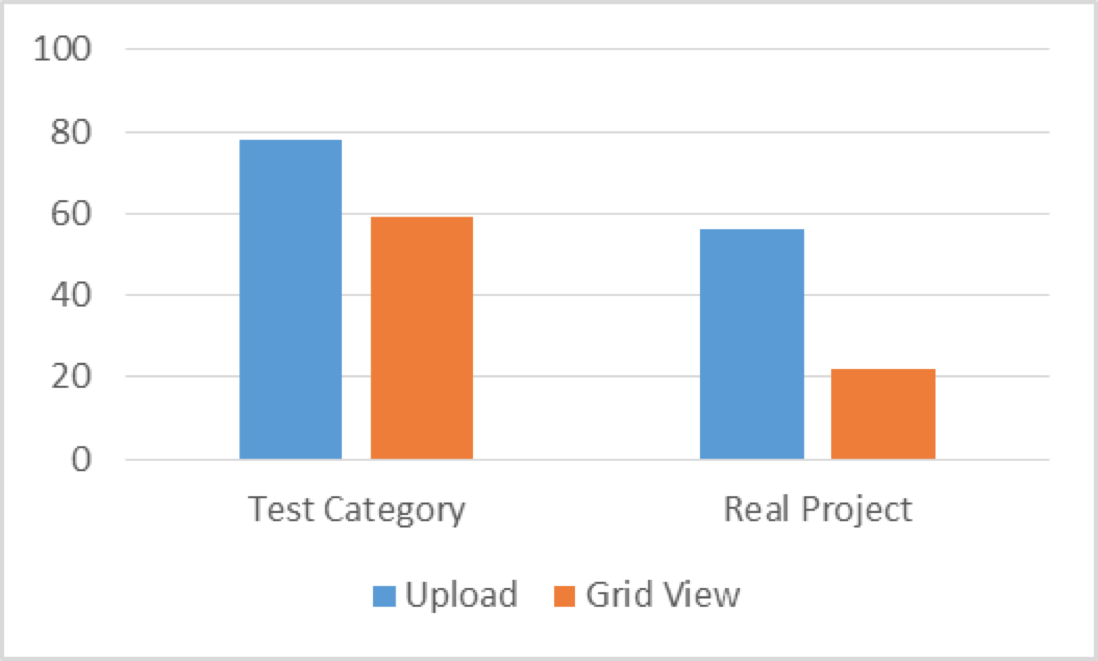
\includegraphics[width=10cm]{./image/D-4-Fig10.png}
  \caption{Finding the remainder of each data pattebrn between Test-Category and the real project.}
  \label{fig:D-4-Fig10}
  \end{center}
   \end{figure}


現実のプロジェクトにて不足していた仕様項目には,論理的機能構造の要素別に見てもInput Adjustment, Output Adjustmentといったメッセージが現れることや入力制御といった単純なことを確認する仕様項目でも漏れているものもあることが確認できる.
一般的に,仕様項目のリストを作成せずにテストケースを作った場合,テストケースのままでは数量の多さから網羅すべき仕様項目の見易さが低下するため,仕様項目の数が不足することが多い.
実験結果も同様の傾向となった.

\section{データ共有タスク間の順序組合せテストケース抽出手法} \label{chap:5}
\subsection{研究の概要} \label{sec:5-1}
\subsubsection{研究の目的} \label{sec:5-1-1}
これまでの研究にて、テストカテゴリを使ったブラックボックステストのためのテスト分析手法を提案してきた。
テストカテゴリを使ったテスト分析では、論理的機能構造という参照モデルを使う。
モデルの要素である入力調整,出力調整,変換,貯蔵、サポート、相互作用でテスト対象をカテゴライズしてテスト条件を特定する。
入力調整,出力調整,変換,貯蔵は、外部観察可能な単一の入出力のみを考慮している分類であり,既出の研究て提案したI/O テストデータパターンで網羅することができる。
しかし、サポートと相互作用は,単一の入出力だけではテスト条件の抽出が出来ない。
なぜなら,サポートと相互作用は,単一の入出力だけではなく,関係する他の処理の呼び出しに着目してテスト条件を抽出するための分類であり,統合して確認すべきテスト条件の抽出が必要だからである。
テストケース数の増加は,単一機能のテストより機能間の統合において問題となる。
この場合のテストケース数は,単一の機能や制御構造の和で求めるのではなく,積となるためである。
それに加え,このテストでは,状態遷移に伴う時系列の組合せのテストも求められることから,テストケース数の爆発問題が生じる。
必要なテストケースの抽出方法とその網羅性に関する研究は多々あるが,多くは機能や制御構造を基にした方法である\cite{Myers,Lee,Grinda,Ostrand}。
状態遷移間の組合せについてはNスイッチカバレージに従ってテストケースを抽出する方法がある。
Nスイッチカバレージとは,状態の遷移をパスとし,N+1個の遷移パスを網羅する基準に従て組合せテストケースを作成する。
N=0では遷移パスの組合せをテストできないためN=1,すなわちS1網羅基準(1スイッチカバレージ)が必要とされている\cite{Beizer}。
しかし,S1網羅基準を満たすテストケース数は,2つの状態遷移間における遷移数の積となり,膨大なテスト工数を必要とする課題になる。
本論文では,機能間の統合における状態遷移間の組合せに着目する。

\subsubsection{テストケース抽出方法と課題} \label{sec:5-1-2}

S1 網羅基準の課題に対す るアプローチとしては,テストケース数を削減する研究と, 自動化により工数を削減する先行研究がある。
自動化による工数削減の研究は,N-スイッチカバレージ を満たすテストケースを形式仕様から自動生成する方法が 知られている。
この方法は,テスト対象となる IT システム の動作を正確に記述したモデルを定義し,そのモデルから 特定の長さの連続した遷移を抽出する方法である (14) 。
対象システムが運動方程式などに従う一般的なモデルベー ステストと異なり,状態遷移にて生ずるシステムの動的な 振舞いを形式仕様化する必要があり,それが困難であるこ とから一般的な IT システムで適用された例は見当たらない。
生成されるテストケース数は N-スイッチカバレージと 同じであり削減されないので,テストケースが自動抽出さ れても,実行のための操作は人手に頼る部分が残り,作業 工数を合理化できない課題がある。
テストケース数を削減する研究としては,状態遷移の組 合せに対して直交表を応用し2因子間の組合せを中心に, 一部3因子の組合せも抽出する研究がある (15) (16) 。
この方法 は,決定表を用いて機械的に組合せを抽出でき,2 因子間 の組合せ即ち S0 網羅基準は完全に網羅できるが,S1 網羅 基準の網羅は不完全であり,かつその選択基準が用いた直 交表に左右されるため重要なテストケースが漏れる課題が ある。
 本研究は,テストケース数を削減するアプローチに属する。
テストケースを機械的に削減するのでは無く,実践の場における経験から生じるノウハウを用いて削減する。
状態遷移に係る不具合は,定義された状態変数や画面とは別に,内部に保存されたデータが影響していることが知られ ている。
具体的には,状態の制御が状態変数や画面によっ て一意に動作するように設計されていたとしても,内部変 数で保持されたデータが存在すると,これが隠れたサブ状 態となり,設計とは異なる振舞いが生じ不具合となる。
本論文では,このような不具合を見つけ出すために必要なテ ストケースを,DFD,ER 図,CRUD 図といったデータ設計文書を入力情報として使うことで合理的に抽出する方法を提案する。

\subsection{順序組合せによるテストケース抽出法} \label{sec:5-2}
本論文では,状態遷移テスト設計における「S1 網羅基準 ではテストケース数が爆発するが,S0 網羅基準では漏れが 生じる」という課題を解決する手法として順序組合せテス トを提案する。

\subsubsection{順序組合せテストの概要} \label{sec:5-2-1}
提案する手法は,2タスク間の順序組合せを対象とする.
%データストアを共有しないタスク間の組合せは, マルコフ連鎖を前提として順序組合せテストの対象から除外する.
%データストアを共有していないため,画面遷移あるいは状態遷移は独立しており,S0網羅基準にてテストを行えば十分だと考えられるからである.
2タスク間の順序組合せの抽出は以下のルールを適用する.
\subsubsection{ルール1:変更タスクの特定}
ルール1を用いて変更タスクとそのデータストアを特定し,拡張CRUD図の変更タスク部分を作成する.

拡張CRUD図とは,テストベースとして与えられたDFD,ER図,CRUD図から$P\{Ta\}$の各$Ta_i$と関連する$So_k$,そして$P\{Ds\}$となる$Ds_j$の関係を追加して作成したものである.


\subsubsection{ルール2:波及タスクの特定}
ルール2を用いて波及タスク群を特定し,拡張CRUD図へ波及タスク部分を追加し図を完成させる.

先に作成した中間の拡張図から変更タスクの操作が$C$か$U$か$D$であるデータストアに着目する.
着目したデータストアに対してエッジを持つタスクが波及タスクのうち,源泉に出力エッジを持つタスクを波及タスクとして特定する.
特定した波及タスクを拡張CRUD図に追記し完成させる.

完成させた拡張CRUD図の例を表~\ref{excrud}に示す.
% Table generated by Excel2LaTeX from sheet 'Sheet1'
\begin{table}[t]
  \centering
  \caption{完成した拡張CRUD図の例}
    \begin{tabular}{r|r|r|r|r|r|r}
    \multicolumn{1}{c|}{タスク} & \multicolumn{3}{c|}{データストア} & \multicolumn{3}{c}{源泉} \\
\cline{2-7}    \multicolumn{1}{c|}{} & $Ds_1$ & $Ds_2$ & $Ds_3$ & $So_1$ & $So_2$ & $So_3$ \\
    \hline
    \hline
    $Ta_1[St_1]$ & $CU$ &   &   & $In$ &   &  \\
    \hline
    $Ta_3[St_1]$ &   & $C$ &   & $In$ &   &  \\
    \hline
    $Ta_2[St_1]$ & $R$ &   &   &   & $Out$ &  \\
    \hline
    $Ta_5[St_1]$ &   & $R$U &   &   &   & $Out$ \\
    \end{tabular}%
  \label{excrud}%
\end{table}%

\subsubsection{ルール3:順序組合せテストケースの抽出}
拡張CRUD図を基に順序組合せのテストケースを抽出し,テストケース表を作成する.
表 ~\ref{TCLISTSAMPLE}にその例を示す.概要の部分は,当該組合せが持つ入力の条件や出力の特性を仕様から抜き出して記載する.

%--------------------------------

%\end{enumerate}

% Table generated by Excel2LaTeX from sheet 'Sheet1'
\begin{table}[t]
  \centering
  \caption{順序組合せテストによる論理的テストケースの例}
    \begin{tabular}{l|l|l}
    No & 論理的テストケース & 順序組合せ \\
    \hline
    1 & 概要 & $Ta_1C \rightarrow Ta_2R$ \\
    \hline
    2 & 概要 & $Ta_1U \rightarrow Ta_2R$ \\
    \hline
    3 & 概要 & $Ta_3C \rightarrow Ta_2R$ \\
    \hline
    4 & 概要 & $Ta_3C \rightarrow Ta_2U$ \\
    \hline
    \end{tabular}%
\label{TCLISTSAMPLE}
\end{table}%


以上の手順で,順序組合せテストに必要なテストケースを抽出する.

\subsection{評価実験} \label{sec:5-3}
\subsubsection{実験の概要} \label{sec:5-3-1}

本節では,旅行代理店向けフライト予約システムの仕様を用いて,3章で述べた実施手順を適用し,順序組合せが抽出できることを確認する.
%本論文では,表~\ref{Featurelist}の新規フライト予約を,変更が入った機能セットとする.
%新規フライト予約からテストケースを抽出するための前提として用意した仕様は,新規フライト予約に関連するDFDとER図(図~\ref{fig:DFD}),CRUD図(表~\ref{CRUD})とする.
%%DFDに含まれるタスク数 $N$は6,データストア数$M$は2,源泉数$L$は4である.



\subsubsection{序組合せテストの適用評価} \label{sec:5-2-2}
次に提案手法で抽出したタスク間の順序組合せと既出の状態を含む$AP$のテストケースを設計する手法である状態遷移テストで,抽出されるテストケースの比較を行う.状態遷移テストのテストベースとなるフライト予約システムの画面遷移図
%である図~\ref{fig:STD}
を使って,順序組合せが確認できる網羅基準であるS1網羅基準を適用する.
%図~\ref{fig:STD}は,
適用範囲を合わせるために,4章の適用のためのサブセットである新規フライト予約を行うために必要な画面と隣接する画面遷移に該当する範囲の図となっている.
仕様の詳細度合いは,DFD,ER図,CRUD図と画面遷移図では同等にしている.
%それは,画面遷移のイベントでのガード条件に記載したデータがDFDのエッジに記載したデータ,ER図のエンティティの属性と一致していることから確認できる.
S1網羅基準を適用すると28の状態遷移パスとなる.
%この表の提案手法の列には,提案手法で抽出した順序組合せに該当する順序組合せを示した.
%状態遷移パスに対応する提案手法で抽出した順序組合せは28のうち,表~\ref{TCLIST2}テストケースNo.1,2,4,5の4つであった.3-25対応
28の状態遷移パスのうち,対応する提案手法で抽出した順序組合せは,
%表~\ref{TCLIST2}テストケースNo.1,2,4,5の
4つであった.
これらは,本状態遷移図のフライト予約状態での登録イベントを起点にするもののみであった.
順序組合せに該当しない状態遷移パスは,互いのタスクで同一のデータを介して処理をするといったことがない.
例えば,フライト検索をした後にキャンセルをするとフライト予約画面に遷移するパスは,前の処理の結果によって影響を及ぼさない.

S1網羅基準では抽出できないが,本手法によって抽出できたテストケースは,

別の機能セットに含まれるタスクであるため,画面遷移図の網羅では現れない.


\section{結論} \label{chap:6}

本研究では研究を行った.

3章では,検証実験にて,本手法の説明を参加者にすることによる仕様項目の一貫性と特定する量の向上が観察できた.更にI/Oデータパターンを使った実験結果の分析によって,実験結果の一部が本手法で提唱している仮説と一致することを観察できた.更に高精度に傾向を分析するため,更なる検証実験は必要である.以降のこの手法の効果と関連する要因とその傾向に対する深い理解とそのための更なる実験をすることで,AUTとフォールトの知識をベースにしたテストカテゴリを作るためのルールをより洗練できると考えている.


\ref{chap:4}章では,テスト実行時のデータI/Oの要素で分類し網羅的に分析する方法を提案した.そして,現場のテストプロジェクトのテストケースを使い,提案した方法の実証を試みた.結果的に,提案した方法で特定した仕様項目と実プロジェクトで作られるテストケースと比較して,不足している仕様項目の発見が可能であることが確認できた.

\ref{chap:5}章では,状態遷移を持つソフトウェアにおいて,変更による変更波及がデータベースや外部変数などの保持データを介して生ずる場合のテストに関して,その網羅基準と,順序組合せテストケースを抽出する手法としてIDAU法を提案した.
DFD,ER図、CRUD図をテストベースとして,3つのルールを適用することでテストが必要な順序組合せを抽出できることを説明した.
提案した手法で組合せが抽出できることを確認するため,フライト予約システムの仕様を具体例にして適用を行った.
最後に従来手法である画面遷移図からS1網羅基準にて抽出した状態遷移パスと提案手法を比較して,テストケース数の削減ができる効果と,S1レベルの画面遷移の網羅では抽出できないテストケースが抽出できる効果を示した.

\nocite{*}
\bibliography{mybib1}
\bibliographystyle{junsrt}

\end{document}
